\documentclass{ecai2010}
\usepackage{times}
\usepackage{graphicx}
\usepackage{latexsym, epstopdf, pgfplots, setspace, units}
\usepackage[algo2e, noend, noline, linesnumbered]{algorithm2e}
\DontPrintSemicolon
\newcommand{\pushline}{\Indp}% Indent
\newcommand{\popline}{\Indm}
\newcommand{\sgn}{\mathop{\mathrm{sgn}}}
\newcommand{\tuple}[1]{\ensuremath{\left \langle #1 \right \rangle }}
\setlength{\belowcaptionskip}{-15pt}
\ecaisubmission   % inserts page numbers. Use only for submission of paper.
                  % Do NOT use for camera-ready version of paper.

\begin{document}

\title{Quality-based rewards for \\ Monte-Carlo Tree Search simulations}

\author{Tom Pepels \and Marc Lanctot \and Mark~H.~M. Winands \institute{Maastricht University, Department of Knowledge Engineering, Maastricht, The Netherlands, email: \{tom.pepels,marc.lanctot,m.winands\}@maastrichtuniversity.nl} }

\maketitle
\bibliographystyle{ecai2010}

\begin{abstract}
In this paper methods for assessing the a posteriori quality of Monte-Carlo simulations are introduced. We show that altering the rewards of simulated play-outs in Monte-Carlo Tree Search based on their assessed quality improves results in five different two-player games. To achieve these results we propose two novel enhancements, the \emph{Qualitative Bonus} and the \emph{Relative Bonus}. The former relies on an uncomplicated heuristic evaluation of the game's terminal state, whereas and the latter relies on the total number of moves made during a simulation. The proposed enhancements lead to a considerable performance increase in all five domains discussed.
\end{abstract}

%-------------------------------------------------------------------
\section{Introduction}
\label{sec:intro}
Monte-Carlo Tree Search (MCTS) depends on the results of numerous simulations, each of these  consist of two parts, 1) the selection step, where moves are selected and played according to the a selection policy, and 2) the play-out step, where moves are played according to a given simulation strategy. At the end of each play-out a terminal state is reached and the result $r$ is usually expressed numerically in some discrete range, e.g. $r \in [-1, 0, 1]$ a loss, draw or win, respectively, and backpropagated along the tree from the expanded leaf to the root node. All rewards are colleced at the nodes on the first ply, on which the final move to play is based. which is selected based on either the node with the highest number of visits, the highest average reward, or a combination of these two \cite{chaslot2008progressive}. This paper focusses on determining the quality of a simulation based on the terminal state reached. Two methods for assessing the quality of a simulation are proposed based on the length of the simulation $m_{ST}$, and a heuristic evaluation of the terminal state $q$. Moreover, we show that adjusting $r$ in a specific way using  $m_{ST}$ and/or $q$ as variables leads to increased performance in five different two-player games.

Other techniques for rewarding simulations have been proposed \cite{Winands2010a}, where play-outs are cut-off early and their state heuristically evaluated. Furthermore, evaluating the final \emph{score} of a game has shown to improve results in games that base the winning player on the one with the highest score \cite{shibahara2008combining}. However, for some domains a strong heuristic evaluation may not be available or too time-consuming, and certainly not all games determine the winning player on the highest scoring player. Nonetheless, using the straightforward discrete reward $r$, any information other than the win/loss/draw state of the play-out's final position is disregarded. For these reasons, we propose assessing the rewards of play-outs based on any information available at the terminal state.

The paper is structured as follows; first, the general MCTS framework is discussed. Next, two different methods for assessing the quality of play-outs are detailed. In Section \ref{sec:qoreward} explains how rewards can be altered given using the quality measures from the previous section. Followed by pseudo-code outlining the proposed algorithm. Finally the performance of the proposed methods is determined in the experiments section, accompanied by a discussion and conclusion.

%-------------------------------------------------------------------
\section{Monte-Carlo Tree Search}
\label{sec:mcts}
\begin{figure}[ht]
	\centering
	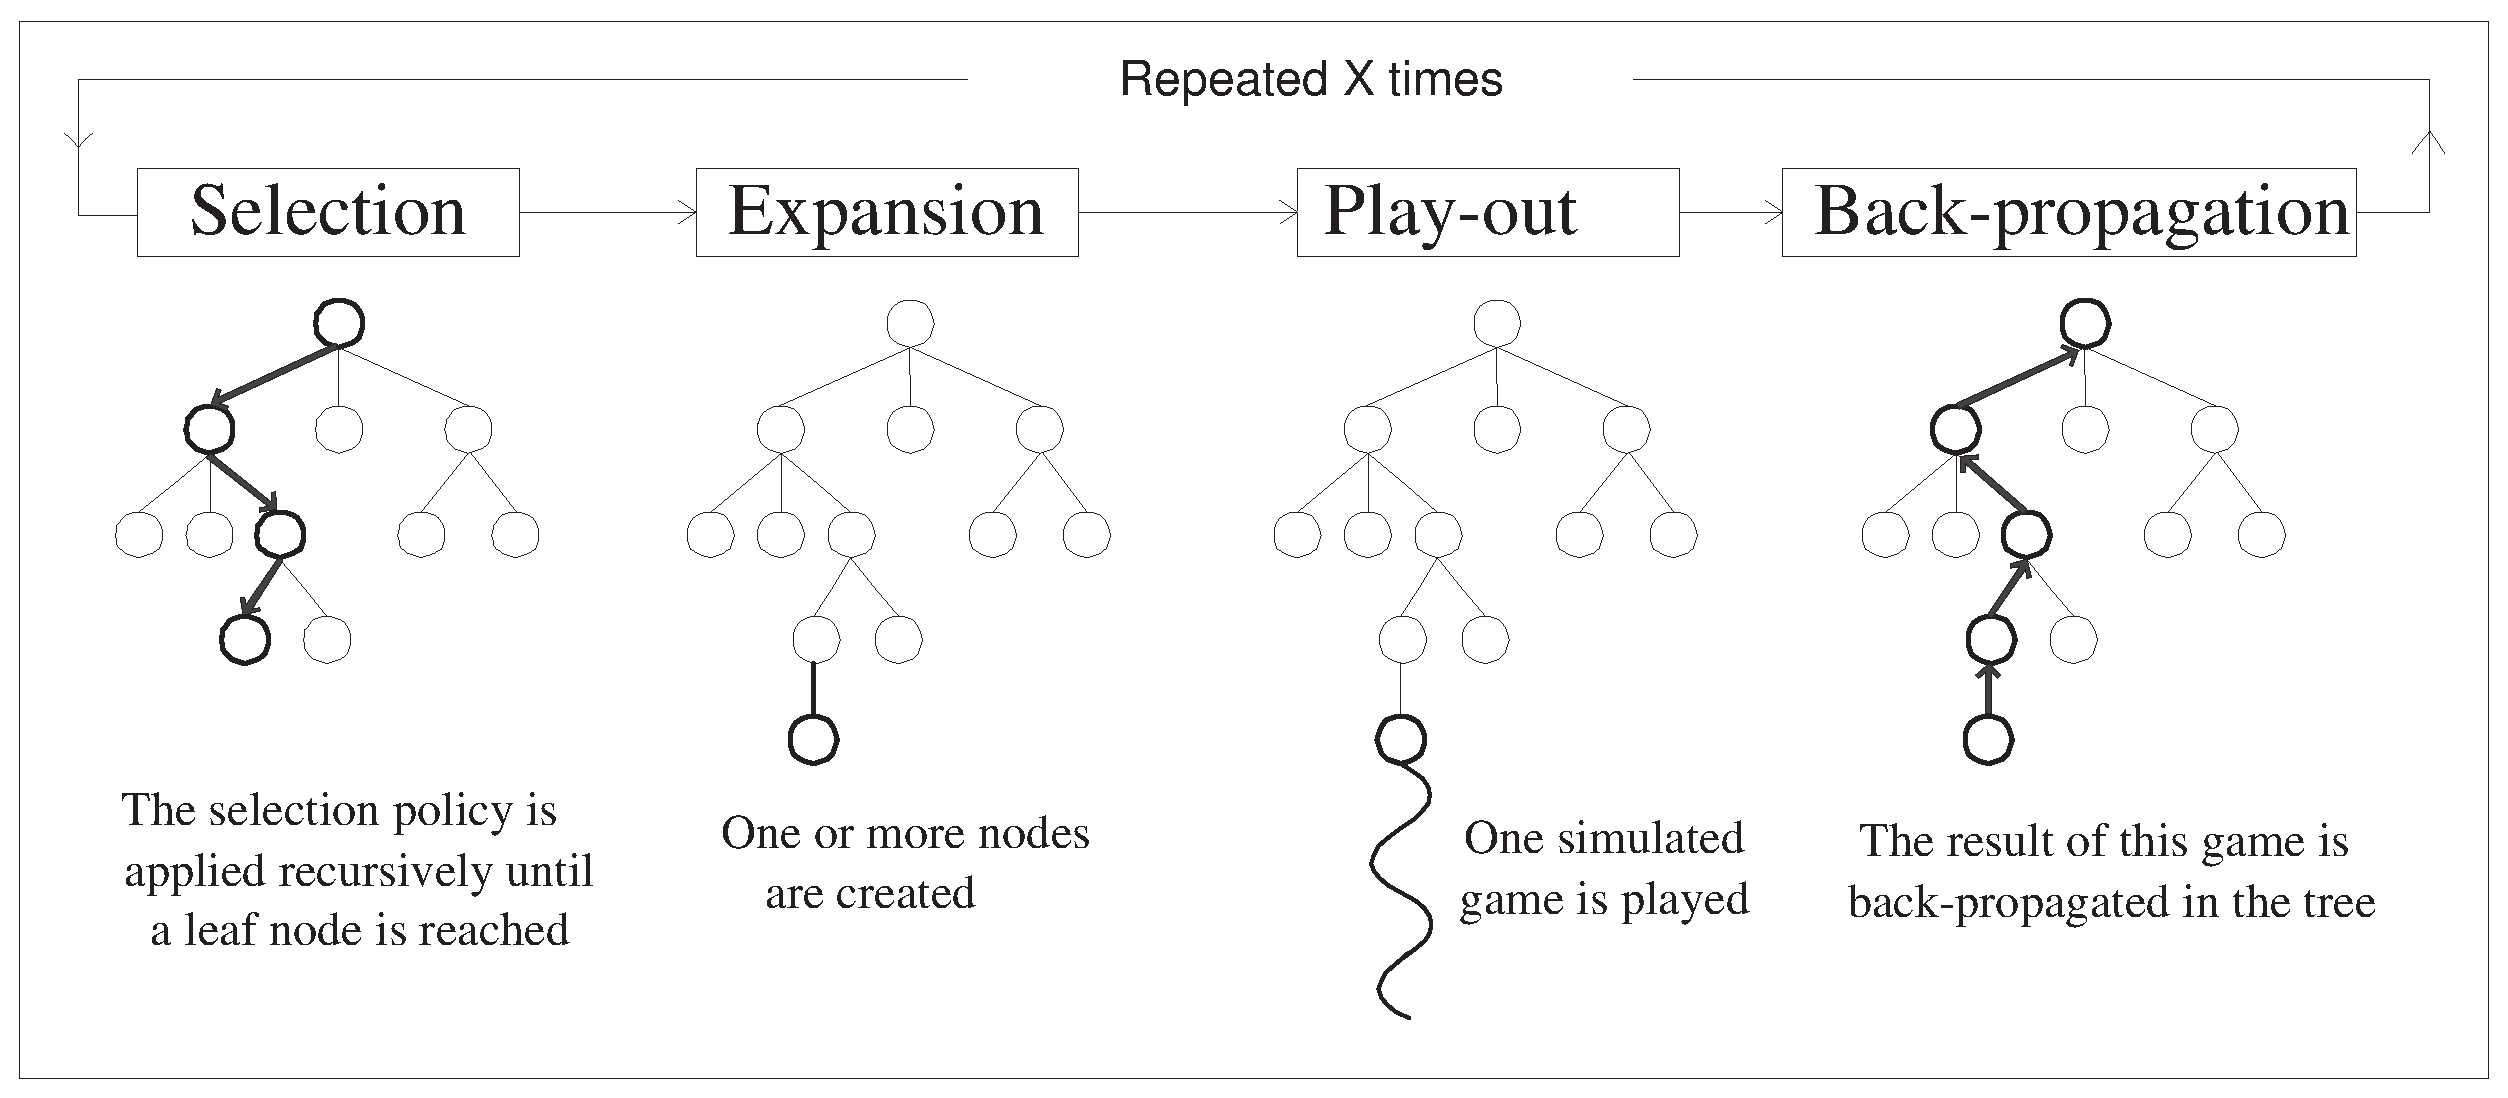
\includegraphics[width=.45\textwidth]{img/figure1.eps}
	\caption{Strategic steps of Monte-Carlo Tree Search \cite{chaslot2008progressive}.}
	\label{fig:mcts-algorithm}
\end{figure}
%from pac-man paper
Monte-Carlo Tree Search (MCTS) is a best-first search method based on random sampling of the state space for a specified domain \cite{kocsis2006bandit},\cite{coulom2007efficient}. In gameplay, this means that decisions are made based on the results of random play-outs. MCTS has been successfully applied to various two-player games games such as Go \cite{lee2010current} and Hex \cite{arneson2010monte}.

In MCTS, a tree is built incrementally over time and maintains statistics at each node corresponding the rewards collected at those nodes and number of times the nodes have been visited. The root of this tree corresponds to the agent's current position. The basic version of MCTS consists of four steps, which are performed iteratively until a computational threshold is reached, i.e. a set number of iterations, an upper limit on memory usage, or a time constraint. The four steps (depicted in Figure \ref{fig:mcts-algorithm}) at each iteration are \cite{chaslot2008progressive}:
\begin{itemize}
\item {\bf Selection}. Starting at the root node, children are chosen according to a selection policy (described in Subsection \ref{subsec:uct}). When a leaf node is reached that does not represent a terminal state it is selected for expansion.
\item {\bf Expansion}. All children are added to the selected leaf node given available moves.
\item {\bf Play-out}. A simulated play-out is run, starting from the state of the added node. Moves are performed randomly or according to a heuristic strategy until a terminal state is reached.
\item {\bf Backpropagation}. The result of the simulated play-out is propagated immediately from the selected node back up to the root node. Statistics are updated along the tree for each node selected during the selection step and visit counts are increased.
\end{itemize}
The combination of moves selected during the selection and play-out steps form a single simulation. In its basic form, MCTS requires no heuristic state evaluation. Nonetheless, in most cases it is beneficial to add some domain knowledge for selecting moves to play during play-out.
% /from pac-man paper

%-------------------------------------------------------------------
\subsection{UCT}
\label{subsec:uct}
%from pac-man paper
During the selection step, a policy is required to explore the tree for rewarding decisions and finally converge to the most rewarding one. The Upper Confidence Bound applied to Trees (UCT) \cite{kocsis2006bandit} is derived from the UCB1 policy \cite{auer2002using} for maximizing the rewards of a multi-armed bandit. UCT balances the exploitation of rewarding nodes whilst allowing exploration of lesser visited nodes. Consider a node $p$ with children $A(p)$, then the policy determining which child $i$ to select:
\begin{equation}
\label{eq:uct}
i^* = argmax_{i \in A(p)}\left\{ v_i + C \sqrt{ \frac{\ln{n_p}}{n_i}}\right\}
\end{equation}
where $v_i$ is the score of the child $i$ based on the average result of simulations that visited it. $n_p$ is the visit count of the node and $n_i$ the visit count of the current child. $C$ is the exploration constant to be determined by experimentation.
% /from pac-man paper

\section{Assessing play-out quality}
\label{sec:poqual}

In this section we will discuss two measures by which the quality of the terminal state of a simulation can be assessed. First, the length of a simulation is detailed as a quality measure, second we consider some heuristic evaluation of terminal states. The next section we establish how these techniques can be used to enhance the rewards of MCTS simulations.

\begin{figure}[ht]
	\centering
	\includegraphics[width=.3\textwidth]{img/figure2.png}
	\caption{A single MCTS simulation \cite{finnsson2010learning}.}
	\label{fig:mcts-simulation}
\end{figure}

The first, straightforward assessment of a play-out's quality is the length of the game played. Consider a single MCTS simulation as depicted in Figure \ref{fig:mcts-simulation}, here we can define two seperate distances: 
\begin{enumerate}
\item The number of moves from the root $S$ to the expanded leaf $N$, $d_{SN}$,
\item The number of moves required to reach $T$, the terminal state, from $N$ during play-out $p_{NT}$.
\end{enumerate}
The length of the simulation is defined as the sum of these distances $m_{ST} = d_{SN} + p_{NT}$, i.e. the total number of moves made by both players to reach the terminal state of the game from the current gamestate. Hence, the length of the simulation can be used as an indicator of the quality of its final result.

Moves selected during play-out are generated by some simulation strategy. Generally this aither a  random strategy, or a rule-based, reactive strategy, combined with a source of randomness such as an $\epsilon$-greedy selection \cite{sutton1998reinforcement, sturtevant2008analysis}. Various alternative methods have been proposed, such as using low-level $\alpha\beta$ searches \cite{winands2011a}, and methods that learn a strategy online, such as N-Grams and the Last-Good-Reply policy \cite{Tak2012}, or the Move-average Sampling Technique (MAST) \cite{finnsson2010learning}. However, each of these methods and strategies have some random element in common. Moreover, they select moves based on some imperfect technique, because they have to make quick decisions to allow for numerous simulations to be made during the allowed time. As such, each move played ultimately increases uncertainty, regarding the accuracy of the final result, by some degree.

A predominant benefit of using simulation length as a quality measure is that it can be determined independent of domain knowledge. Unless the game's length is fixed, the variance of the length of a play-out can be informative in determining its quality. 

%-------------------------------------------------------------------
\section{Quality-based play-out rewards}
\label{sec:qoreward}
Alter rewards, centered around $r$ using sigmoid. Sigmoids are great, i love them, here's why!
\begin{figure}[ht]
\centering
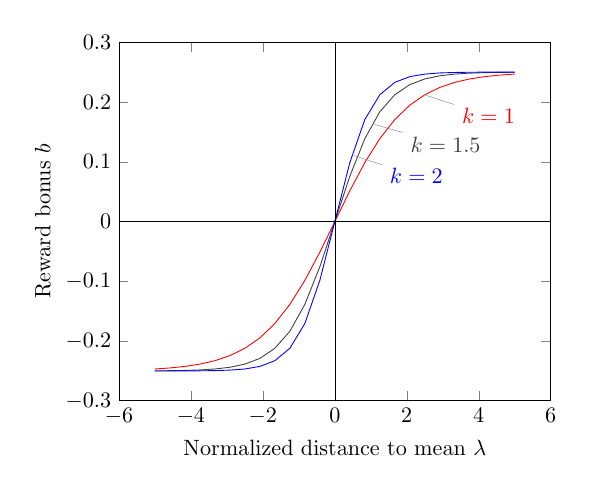
\begin{tikzpicture}[scale=0.8]
\pgfplotsset{compat=1.9}
  \begin{axis}[
	ylabel = Reward bonus $b$,
    xlabel = Normalized distance to mean $\lambda$,
  	axis equal image=false 
  	]

    \addplot[red, mark=none] {.5/(1+e^(-x)) - .25} node [pos=0.75,pin={-10:$k=1$},inner sep=0pt]{};
    \addplot[darkgray, mark=none] {.5/(1+e^(-1.5*x)) - .25} node [pos=0.607,pin={-10:$k=1.5$},inner sep=0pt]{};
    \addplot[blue, mark=none] {.5/(1+e^(-2*x)) - .25} node [pos=0.55,pin={-10:$k=2$},inner sep=0pt]{};
    \draw[ultra thin] (axis cs:\pgfkeysvalueof{/pgfplots/xmin},0) -- (axis cs:\pgfkeysvalueof{/pgfplots/xmax},0);
	\draw[ultra thin] (axis cs:0,\pgfkeysvalueof{/pgfplots/ymin}) -- (axis cs:0,\pgfkeysvalueof{/pgfplots/ymax}); 
  \end{axis}
\end{tikzpicture}
    \caption{Rewards resulting from sigmoid functions centered around 0.}
	\label{fig:sigmoids}
\end{figure}

\subsection{Relative Bonus}
Alter the rewards based on $m_{ST}$

\subsection{Qualitative Bonus}
Alter the reward based on the quality of the terminal state. Different heuristics per game.

%-------------------------------------------------------------------
\section{Pseudo-Code}

Explain all the alterations to standard MCTS

\begin{algorithm2e}[ht]
\setstretch{1.15}
  {\bf MCTS}(node $p$, cumulative node depth $d_{Sp}$):\;
  \pushline
    \If{isLeaf($p$)}{Expand($p$)}
    Select a child $i$ according to Eq.~\ref{eq:uct} 	\;
    $d_{Si} \gets d_{Sp} + 1$								\;
    \eIf{$n_i = 0$}{
    	$\tuple{r, q, p_{iT}} \gets$ Playout$(n_i)$ 					\;			\label{alg:results}
    	$m_{ST} \gets d_{Si} + p_{iT}$									\;
    	\If{enabled$(rb)$}{
    		$r \gets r + \sgn(r) \times$ BONUS$(\bar{M} - m_{ST}, \hat{\sigma}_m)$ 		\;
    		Update $\bar{M}$ and $\hat{\sigma}_m$ with $m_{ST}$						\;
		}
		\If{enabled$(qb)$} {
    		$r \gets r + \sgn(r) \times$ BONUS$(q -\bar{Q}, \hat{\sigma}_q)$ 		\;
    		Update $\bar{Q}$ and $\hat{\sigma}_q$ with $q$ 						\;
    	}
    	Update node $i$ with $r$
    }{
    	$r$ = -MCTS($i$, $d_{Si})$)								\; 
    }
    Update node $p$ with $r$													\;
   \popline
    {\bf return} $r$													\;
  	\;
    {\bf BONUS}(distance to mean $\delta$, sample std. dev. $\hat{\sigma}$):			\;
    \pushline
    	$\lambda \gets \nicefrac{\delta}{\hat{\sigma}}$								\;
    	$b \gets \nicefrac{0.5}{\left(1+\exp(-K\lambda)\right)} - 0.25$					\;
    \popline
    \bf{return} $b$														\;
  \vspace{0.3cm}
  \caption{Pseudo-code of the MCTS and BONUS functions \label{alg}}
\end{algorithm2e}

%-------------------------------------------------------------------
\section{Experiments}
Experiments run on 5 different two-player games.
\subsection{Experimental setup}
Describe setup of experiments, k's used, c's used.

\subsection{Results}
- Results UCT vs RB
- Results UCT vs QB
- Results UCT vs RB + RB
- Results RB vs QB
- Graph of K's / UCT C's

%-------------------------------------------------------------------
\section{Conclusion}
Relative bonus - interesting because requires no domain knowledge, works best in games with long play-outs.
QB works in all domains, but requires domain knowledge, nonetheless, even using simple evaluation of the terminal state improved results considerably.

RB especially interesting for General Game Playing (GGP), where knowledge of games is sparse. RB improves results without domain-dependent knowledge.

Would be interesting to determine if RB/QB could improve results in non-game domains.

%-------------------------------------------------------------------
\subsection*{Acknowledgments}
This work is partially funded by Scientific Research (NWO) in the framework of the project Go4Nature, grant number 612.000.938.
\bibliography{references}
\end{document}